\documentclass[a4paper,11pt, onecolumn]{article}

    \usepackage{indentfirst}
    \usepackage{amsmath}
    \DeclareMathOperator\arctanh{arctanh}
    \usepackage{xcolor, graphicx}
    \usepackage{wrapfig}
    \usepackage{caption} 
    \captionsetup{justification=justified}
    \usepackage{appendix}
    \usepackage{textcomp}
    \usepackage{natbib}
    \setlength{\bibsep}{1pt}
    
    \setlength{\textheight}{21cm}
    \setlength{\textwidth}{15cm}
    \setlength{\hoffset}{-0.5in}

     

% define the title

\title{\vspace{-0.3 in} An Investigation into the Natural Width of the Semi-Classical Jet Reclustering Algorithm using Monte Carlo Simulation \vspace{-1ex}}
\author{Candidate Number: 676225  \hspace{1in}     Word Count: 0000}
\date{\vspace{-2ex}\hspace{-0.25in}Supervisor: Dr. J. Tseng \hspace{1.2in} Project: PP0804 }
	

\begin{document}

    \maketitle
    \vspace{-1cm}
    \begin{abstract}
     
         \normalsize
         Using Monte Carlo simulations of $Z' \to u + \bar{u}$, I investigated the widths of jets reconstructed by the Semi-Classical sequential recombination
         algorithm in comparison to other existing jet reclustering algorithms. I found that the Semi-Classical algorithm
         is effective at reconstructing the 60\% jet width for a jet width parameter, $R = 1.5-2.0$; where existing algorithms are effective
         for $R = 0.5-1.0$.
   
    \end{abstract}


\section*{Introduction}

 In high energy physics, jets are narrow beams of propagating high energy hadrons. 
 The production of jets is a common process in high energy elementary particle collisions. Jets are typically 
 produced by an interaction that contains free quarks or gluons in its final state, such as the decay of a $Z_0$ boson into two quarks. When 
 the free quarks and gluons separate to a distance of order 1 fm the strong force will become large, which will decelerate the coloured
 objects rapidly. This deceleration will cause them to radiate hadrons (mostly light $\pi$-mesons), similar to how a decelerated charge will radiate photons through 
 bremsstrahlung. As the original quark or gluon will have been boosted, the radiated hadrons will be collimated due to the relativistic headlight 
 effect, forming the narrow beam of hadrons that we call a jet. A qualitative description can be found on p 18-19 of \cite{HalzenMartin}. \newline

 Jets produced at high energy collider experiments are detected when the light hadron constituents of the jets deposit energy
 into the hadronic calorimeter. To analyse events containing jets, one must use a reclustering algorithm to reconstruct 
 the jets, which means to identify the energy deposits caused by the jet constituents and sum them to find the total jet 4-momentum.
 One set of reclustering algorithms are the sequential recombination algorithms, which selectively add together the calorimeter energy deposits to form the jet.
 In this report I consider a new sequential recombination algorithm, the Semi-Classical(SC)
 jet algorithm \cite{sc}, in comparison to the three most commonly used sequential recombination algorithms;
 the $k_t$, the anti-$k_t$ and the Cambridge-Aachen(CA) algorithms \cite{salam}. \newline

 The latter three algorithms begin with a set of 4-vectors (clusters) which represent the energy deposits in the calorimeter. One then introduces an inter-jet distance between
 clusters $i$ and $j$ defined as,
 \begin{equation}
   d_{ij} = \text{min}
[(p_{ Ti})^a, (p_{ Tj})^a]  \left(\frac{\Delta  R_{ij}}{R}\right) ^2, \hspace{1cm} \Delta R_{ij} = \sqrt{(y_{i} - y_{j})^2 + (\phi_{i} - \phi_{j})^2} \label{dij}
 \end{equation}
 \noindent and a particle-beam distance for cluster $i$ defined as,
 \begin{equation}
   d_{iB} = (p_{Ti})^a \label{diB}
 \end{equation}
 where $y = \frac{1}{2}\ln[(E+p_Z)/(E-p_Z)]$ \footnote{We are using natural units where c = 1, hence momentum can be expressed in units of energy.}
 is rapidity (as defined in \S2.3 of \cite{wong}), $\phi$ is azimuthal angle, $p_T$ is transverse momentum (component of momentum perpendicular to the beam-pipe
 of colliding particles) and $p_z$ is the component of momentum that is parallel to the beam-pipe of colliding particles
 \footnote{A diagram to show the beam-pipe of colliding particles and the use of angular coordinates in the context of a typical collider experiment is shown in Appendix \ref{coordinates}.}.
 $R$ is the jet width parameter, which is a free parameter of the algorithm. I will discuss the significance of this parameter below. \\

 The inter-jet and particle-beam distances are not physical distances as such, but can instead be thought of as dimensionful measures of how likely it is that
 clusters $i$ and $j$ represent energy deposits caused by hadrons from the same jet. If the inter-jet distance for a pair of clusters is smaller than the particle-beam distances
 for the two clusters ($d_{ij} < d_{iB}$) 
 then it is likely that the two clusters are from the same jet. 
 In contrast, if $d_{ij} > d_{iB}$ then it is unlikely that the two clusters are from the same jet.\\
 
 \noindent The algorithm then follows the steps
   \begin{quote}
   1. Calculate $d_{ij}$ and $d_{iB}$ for all combinations of clusters. \newline 
   2. Find the minimum of the $d_{ij}$ and $d_{iB}$. \newline
   3. If the minimum is a $d_{ij}$ combine cluster $i$ and $j$ to form a new cluster and return to step 1. \newline
   4. If the minimum is a $d_{iB}$ then call cluster $i$ a final-state jet, remove it from the set and return to step 1.  \newline
   5. Stop when all clusters have been declared as jets. 
   \end{quote} 
 The parameter $a$ in Eq. \eqref{dij} and \eqref{diB} takes the value $a = 2$ for the $k_t$ algorithm, $a = -2$ for the anti-$k_t$ algorithm 
 and  $a = 0$ for the Cambridge-Aachen algorithm \cite{salam}. \newline

 The Semi-Classical jet algorithm \cite{sc} is a modified sequential recombination algorithm. This algorithm follows the same steps as outlined
 above but, instead of using Eqns. \eqref{dij} and \eqref{diB}, we use the redefined inter-jet and particle beam distances
 \begin{equation}
   d_{ij} = \frac{1}{4} (m_{Ti} + m_{Tj})^2 \left( \frac{\Delta R_{ij}}{R} \right) ^3 \label{dij sc}
 \end{equation}
 \begin{equation}
   d_{iB} = m_{Ti}^2 \label{diB sc}
  \end{equation}
  where $m_{Ti} = \sqrt{p_{Ti}^2 + m_i^2}$ is the transverse mass of cluster $i$, and $m_i$ is its mass. The algorithm is formed by considering the angular distribution
  of radiation being  classically emitted by a moving charge, which contains a relativistic boost factor $\gamma \sim E_i + E_j$. This boost factor is then modified so it
  contains only longitudinally invariant quantities, which are quantities that are invariant under Lorentz boost transforms along the beam-pipe of the
  colliding particles, thus the boost factor becomes $\gamma \sim m_{Ti} + m_{Tj}$. The algorithm has been shown to effectively subtract background as it reconstructs the jet \cite{sc},
  in a manner that is similar to a process called ``pruning'', which is a background subtraction technique often applied to reconstructed jets formed by sequential 
  recombination algorithms \cite{pruning}. However, this pruning nature of the SC jet algorithm can also remove genuine jet constituents as well.  
  \newline

  In this report I will investigate how the sequential recombination algorithms listed above reconstruct the width of jets. This is important as in 
  the inter-jet distances, defined in Eqns. \eqref{dij} and \eqref{dij sc}, the jet width parameter, $R$, effectively gives the maximum width of a reconstructed jet.
  This is because when $\Delta R_{ij} > R$ for a pair of clusters, we will find that $d_{iB} < d_{ij}$ for the cluster with the smaller value of ${p_T}$ or ${m_T}$.
  Hence, the algorithm will never merge these two clusters as it will always skip to step 4 of the algorithm and remove one of the clusters as a jet. $R$
  is a free parameter of the algorithms, which means that the user sets the value of $R$. Choosing an appropriate value for $R$ 
  is important in reconstructing jets correctly with minimal background. An $R$ value 
  that is too large may allow too much background to be included in the reconstructed jet, whilst an $R$ that is too small will mean that we may lose
  significant amounts of the actual jet in the reconstruction. By better understanding how the algorithms reconstruct the width of the jet for different values of $R$,
  we will be able to better select the $R$ value to reconstruct the natural width of the jet.
  \newline

  The decay process I used to produce the jets was $Z' \to u + \bar{u}$, where the $Z'$ boson is a hypothetical gauge boson 
  that is predicted by various beyond Standard Model theories \cite{Zprime1, Zprime2, Zprime3}.
  This particular decay was chosen as it is a colourless object that decays with a narrow resonance into two high energy free quarks that will
  form jets. The fact that the $Z'$ boson is a narrow resonance means that the two quarks will be produced with reasonably well-defined energy of $E_q \sim \frac{1}{2} m_{Z'}$. By not considering 
  soft-QCD radiation (radiation caused by strong force interactions with low momentum transfers) and initial state radiation (radiation from the beam of colliding 
  particles) in the simulation I produced events with a low contribution from the underlying event (everything not in the two jets) \cite{underlyingevent}.
  The two quarks also have $\phi$ values differing by $\pi$ because the $Z'$ created would have zero transverse momentum, hence the 
  resulting particles of the decay must also have zero total transverse momentum. The opposite $\phi$ values meant that 
  there was a clear separation between the two jets which was used to differentiate between them. \\

  To conduct these investigations I used Monte Carlo simulations to produce the data sets that the jet reconstructing algorithms were applied to. Monte Carlo
  simulations are a broad set of computational techniques that use random numbers to produce numerical results based on probabilistic distributions.
  Simulations were used to give us the opportunity to apply the algorithms to data sets that are independent of detector effects and where we know the true
  4-momentum of the original quark that caused the jet. However, it must be noted that, whilst simulation is a useful tool in analysing the 
  performance of jet reclustering algorithms, testing with experimental data is also required. \\

  The first section of this report will outline the details  of the simulation and the computational tools used to simulate and analyse the data. 
  The second section will present the analysis of the data in three subsections; firstly I will characterise the distribution of the jet energy from the simulation, 
  then I will consider the width of jets reconstructed using the SC jet algorithm and lastly I will compare the width reconstruction performance of the SC jet algorithm
  to the $k_{T}$, anti-$k_T$ and CA algorithms. 
  In the final section I will present the conclusions of the analysis and outline areas for further research.
 
\section{Simulation} 

  To produce jets for analysis I used the simulation package Pythia, version 8.176, which is a standard tool for creating Monte Carlo simulations of high energy particle 
  collisions  \cite{Pythia}. In the simulated $Z' \to u + \bar{u}$ events, the $Z'$ was produced in a proton-proton collision in the centre of mass frame with a total collision
  energy of 7 TeV. As the mass of the $Z'$ is not a fixed parameter, the value of $m_{Z'}$ could be varied to produce jets with a range of initial quark energies, 
  $E_q$. I generated events for $m_{Z'}$ ranging from 200 to 2000 GeV in steps of 200 GeV, with 100,000 events for each mass. As $E_q \sim \frac{1}{2}m_{Z'}$,
  this range of masses gave me a large sample size of jets with $E_q$ in the range 100-1000 GeV. A cut of $p_T < 100$ GeV was applied to jets reconstructed by
  the algorithms, which is done to reduce the number of background events that are reconstructed as jets by the reclustering algorithms.
  Hence, jets with $E_q <$ 150 GeV were not considered as they will not be consistently reconstructed by the algorithms, so cannot be used to investigate the algorithms. \\

  To analyse these events I used Rivet, version 2.0.0, which is a Monte Carlo validation package \cite{Rivet}.
  Using Rivet I built a programme to analyse the simulations on an event-by-event basis. The Pythia simulation produced a large event-record that contained 
  data on all particles used in the simulation, including a large number of intermediary particles. The Rivet analysis programme extracted the required 
  particles from this event-record using ``projections'', which are objects in the Rivet computing infrastructure. 
  My analysis programme used the visible final state projection, which outputs the 4-momentum of all long-lived particles in the final state excluding neutrinos. I also used
  projections from the FastJets package, version 3.0.4, to apply the various jet reclustering algorithms to the particles from the visible final state projection \cite{FastJets}.
  I was able to extract the 4-momentum of the initial quarks from the Pythia event-record within the analysis.\\

  A problem I encountered was that Rivet's internal plotting package, YODA, was not able to produce many of the data plots required,
  in particular 2D histograms. To overcome this problem I was able to interface the Rivet analysis package with ROOT, which is a standard analysis and plotting 
  package used in high energy physics analyses \cite{ROOT}. 

\section{Analysis}
\subsection{Characterising the Jet Width} \label{ss fs}
  
  In this subsection I will characterise the true width of the jets by considering the final state particles, as selected by the visible final
  state projection. This characterisation I will call the final state jet widths, which will be used as a benchmark to compare the width reconstruction of
  jet reclustering algorithms to.
  Figure \ref{detector_quark} shows the positional distribution of final-state particle energies alongside the position of the
  initial quarks from the $Z'$ decay for a single event. The x-axis represents pseudorapidity, defined as 
  $\eta = -\ln\left[\tan\left(\theta /2 \right)\right]$, as done in \S2.4 of \cite{wong}, where $\theta$ is the polar angle to the beam-pipe of the colliding 
  particles\footnote{A diagram to show the beam-pipe of colliding particles and the use of angular coordinates in context 
  of a typical collider experiment is shown in Appendix \ref{coordinates}.}. Pseudorapidity is used as it is a
  quantity that is mathematically similar to rapidity, $y$, in the high energy limit
  \footnote{The high energy limit is when $E \gg m$, where $E$ is the energy and $m$ is the mass of particle.} \cite{pseudorapidity},
  but calculable from just the polar angle. In Figure \ref{detector_quark} 
  we can see that most of the final state energy has been deposited in the jets (the clusters of energy around the initial quark position). We can also see that much 
  of the background energy from the underlying event is at high absolute values of $\eta$. Hence, a pseudorapidity cut of $\eta < |2|$ was applied to reduce this background.


  \vspace{-0.12cm}
  \begin{figure}[h]
    \begin{center}
      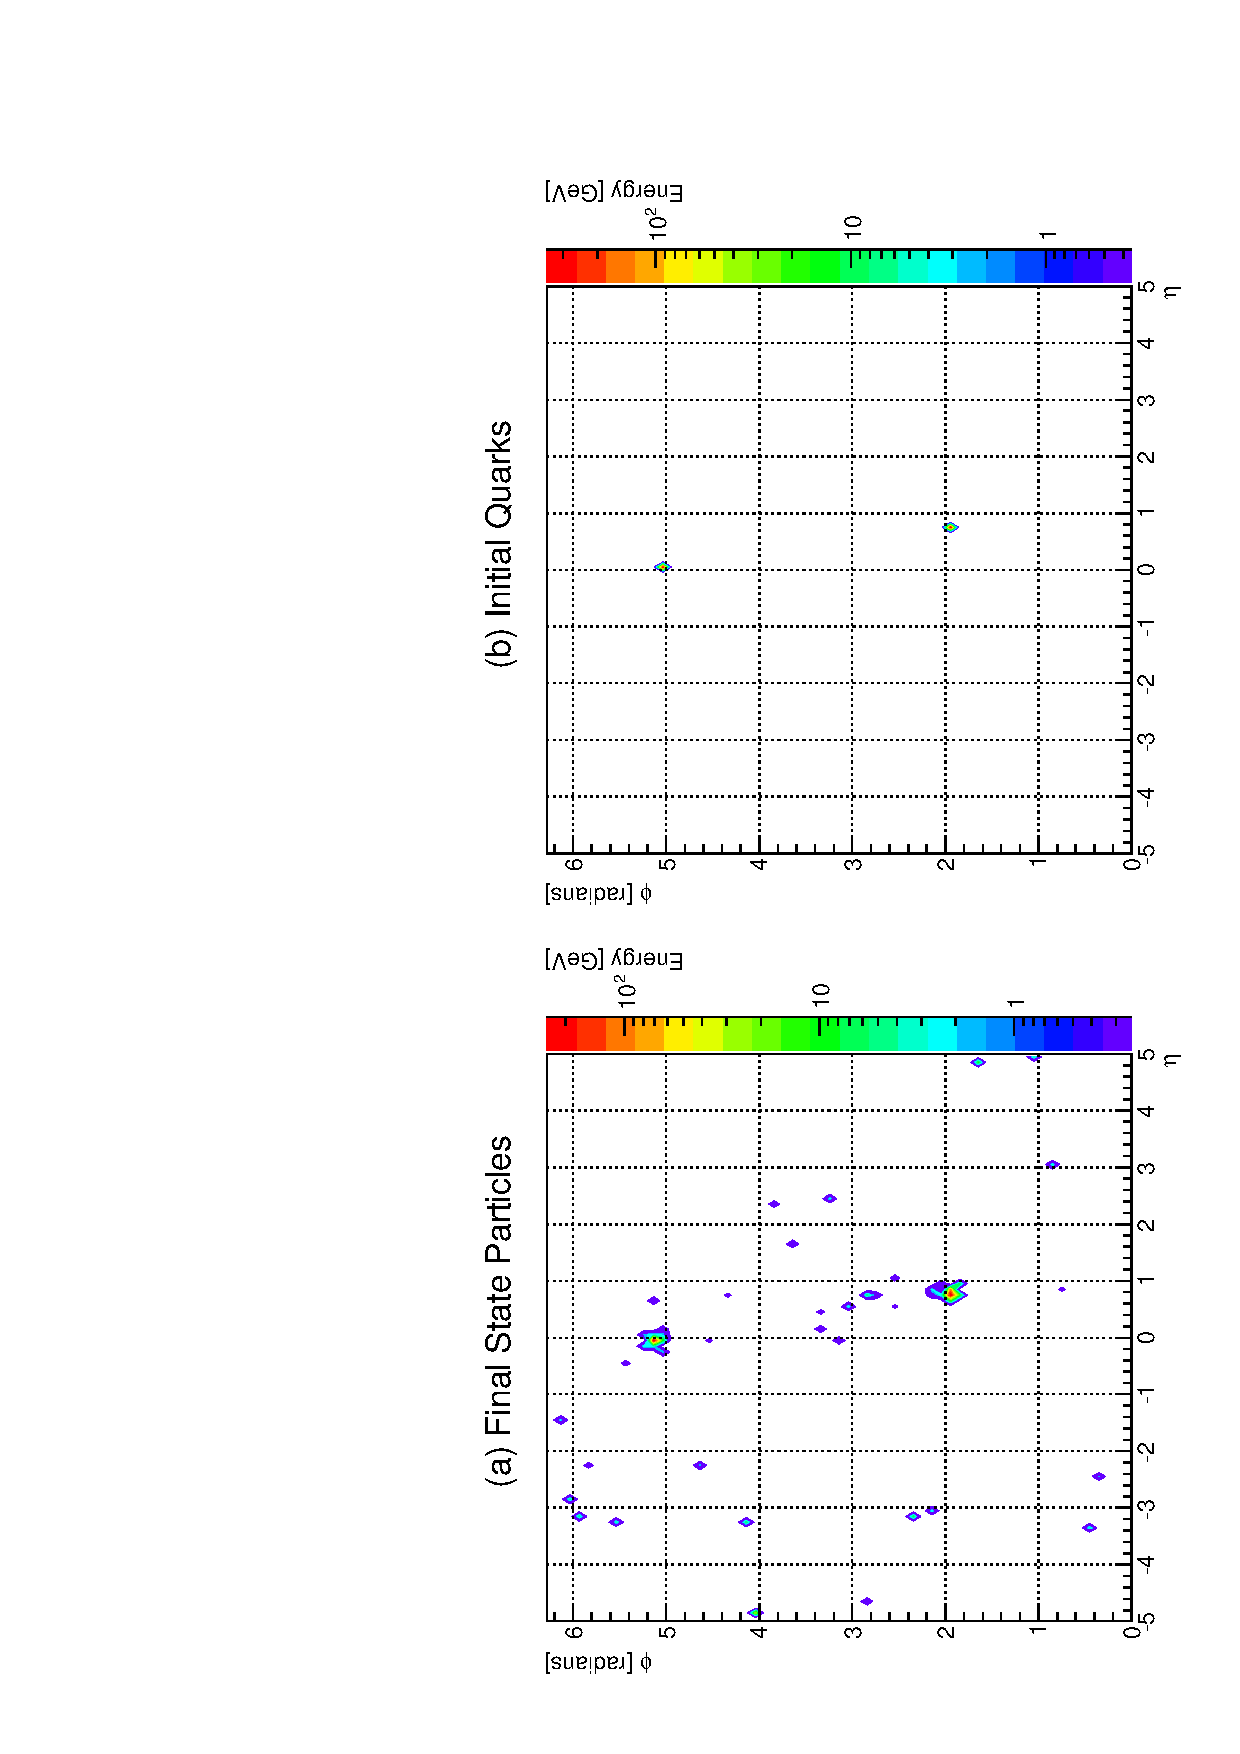
\includegraphics[width = 0.95\textwidth]{detector_quark}
      \caption{A single event energy distribution of (a) the final state particles (b) the initial quarks on an $\eta$-$\phi$ grid
           with a resolution of 0.1. The energy axis is a log-scale for both plots.}
      \label{detector_quark}
    \end{center}
  \end{figure}

  \vspace{-0.4cm}

  As the two quarks are clearly separated in $\phi$-space, analysis of the width of the jets was done using $\phi$ to prevent a contribution from the opposite jet. 
  Figure \ref{lego_plot} is a 2D histogram, containing final state particles from all events, that shows the $\phi$ distribution of the final state
  particles about the initial quark axis, weighted by the final state particle energy, for different values of initial quark energy. 
  This distribution has been normalised by the quark energy.
  The figure effectively gives the azimuthal energy profile of the average jet produced. The distribution shows that jets become thinner at higher energies and 
  their widths are on the scale 0.01-0.1 radians.
  
  
  \vspace{+0.05cm}
  \begin{figure}[ht]
    \begin{center}
      \includegraphics[width = 0.6\textwidth]{lego_plot}
      \caption{The normalised $\phi$ distribution of final state energy about the quark axis for different values of quark energy, $E_{q}$.
               The distributions were normalised by $E_{q}$}
      \label{lego_plot}
    \end{center}
  \end{figure}
  \vspace{-0.25cm}

  Figure \ref{lego_plot} gives us an idea of the shape of the final state jets in $\phi$-space. However, it is required that information about the width of these 
  jets is quantised, to be able to compare to the widths of the jets reconstructed by the reclustering algorithms later. This is done by finding the value of 
  $\Delta\phi$ that contains 60\% and 95\% of the initial quark energy in the final state as a function $E_{q}$. I will call these values $r_{60}$ and $r_{95}$ 
  respectively. \\
  
  The technique used to calculate the $r_{60}$ and $r_{95}$ values goes as follows; first sum the energies of final state particles close to the 
  quark axis in $\phi$ to find the values of $r_{60}$ and $r_{95}$ for each individual jet. 
  The distributions of the individual $r_{60}$ and $r_{95}$ are calculated for quark energies 200-1000 
  GeV with bins of width 100 GeV. Figure \ref{r q distr} shows these distributions for the quark energies of 200, 600 and 1000 GeV.
  We can see that the distributions consist of a peak with a long tail. By defining a value of skewness using Eq. (14.1.5) of \cite{skewness} as,
  \begin{equation}
    \text{Skew}(x_1 ... x_N)  = \frac{1}{N} \sum\limits_{j=1}^N \left[\frac{x_j - \bar{x}}{\sigma}\right]^3   \label{skew}
  \end{equation}
  I found that the $r_{60}$ distributions have skewness values in the range 2.3 - 3.3 and the $r_{95}$ distributions have skewness values in the range
  1.5-2. The large skewness values indicate that the mean is not a representative measure of the true jet width, as the mean is being distorted by the large tails
  of the distribution.
  Instead a fifth-order polynomial was used to fit these distributions to identify the maxima; the fitting is shown in Figure \ref{r q distr} by the red line.  
  The values of $r_{60}$ and $r_{95}$ at the maxima are what I shall use to represent the final state jet widths. This fitting
  was done and errors in the values of $r_{60}$ and $r_{95}$ were calculated using the fit capabilities within ROOT.\\

  \begin{figure}[!htb]
    \begin{center}
      \includegraphics[width = \textwidth]{r_q_distr}
      \caption{Histograms to show the final state distributions of $r_{60}$ for initial quark energy, $E_{q}$ = 200, 600 and 1000 GeV [(a), (b) and (c)]
               and $r_{95}$ for $E_{q}$ = 200, 600 and 1000 GeV [(d), (e) and (f)]. A fifth-order polynomial has been
               fitted to these to identify the maxima of the distributions.  \vspace{-0.5cm} }
      \label{r q distr}
    \end{center}
  \end{figure}

  Figure \ref{r q} shows the final state jet widths $r_{60}$ and $r_{95}$ as a function of the quark energy. The errors
  in $r_{60}$ and $r_{95}$ are in the range 1-2\%, error bars are not shown as they are smaller than the size of the square point markers.
  The dotted lines are error weighted fittings of the form $r = A/(E_{q}+B)$, where $A$ and $B$ are fitting parameters. When fitting, each
  data point is weighted with $(1/\Delta r)^2$, where $\Delta r$ is the error in $r_{60}$ or $r_{95}$ for that point. A full list of fitting 
  parameters used is shown in Appendix \ref{fittings}. This fitting form is chosen as jets will narrow due to relativistic effects with the form
  $r \propto 1/p_T$, as described in Eq. (11.43) of \cite{HalzenMartin}. In the high energy limit it is found that $E \sim p$, 
  so the generalised form $p_T = E + B$ can be used. The fitting is good, showing that the distribution of jet widths is consistent with jet width 
  narrowing proportional to inverse-$p_T$. \\
  
  However, one must exercise some caution in declaring the final state jet widths, shown in Figure \ref{r q}, as the absolute true widths of the jets. 
  An effect which could cause the widths to be misrepresentative is that if the free quark loses energy through hard gluon bremsstrahlung \cite{gluonbrem},
  then the energy of the jet may be less than the energy of the initial quark. In this case
  the summation process in the width characterisation will be forced to include some wider angle background to account for the lost quark energy.
  This will cause the $r_{95}$ and $r_{60}$ values to be slightly larger than they should be. In particular the $r_{95}$ value will be sensitive to this
  effect as it is already at the edge of the jet distribution. Although some protection is provided against this widening effect by using the maxima of 
  the fitted distribution, hence excluding the tail where most of the anomalous events will lie, there may still be some effect. \\


  \begin{figure}[!htb]
    \begin{center}
      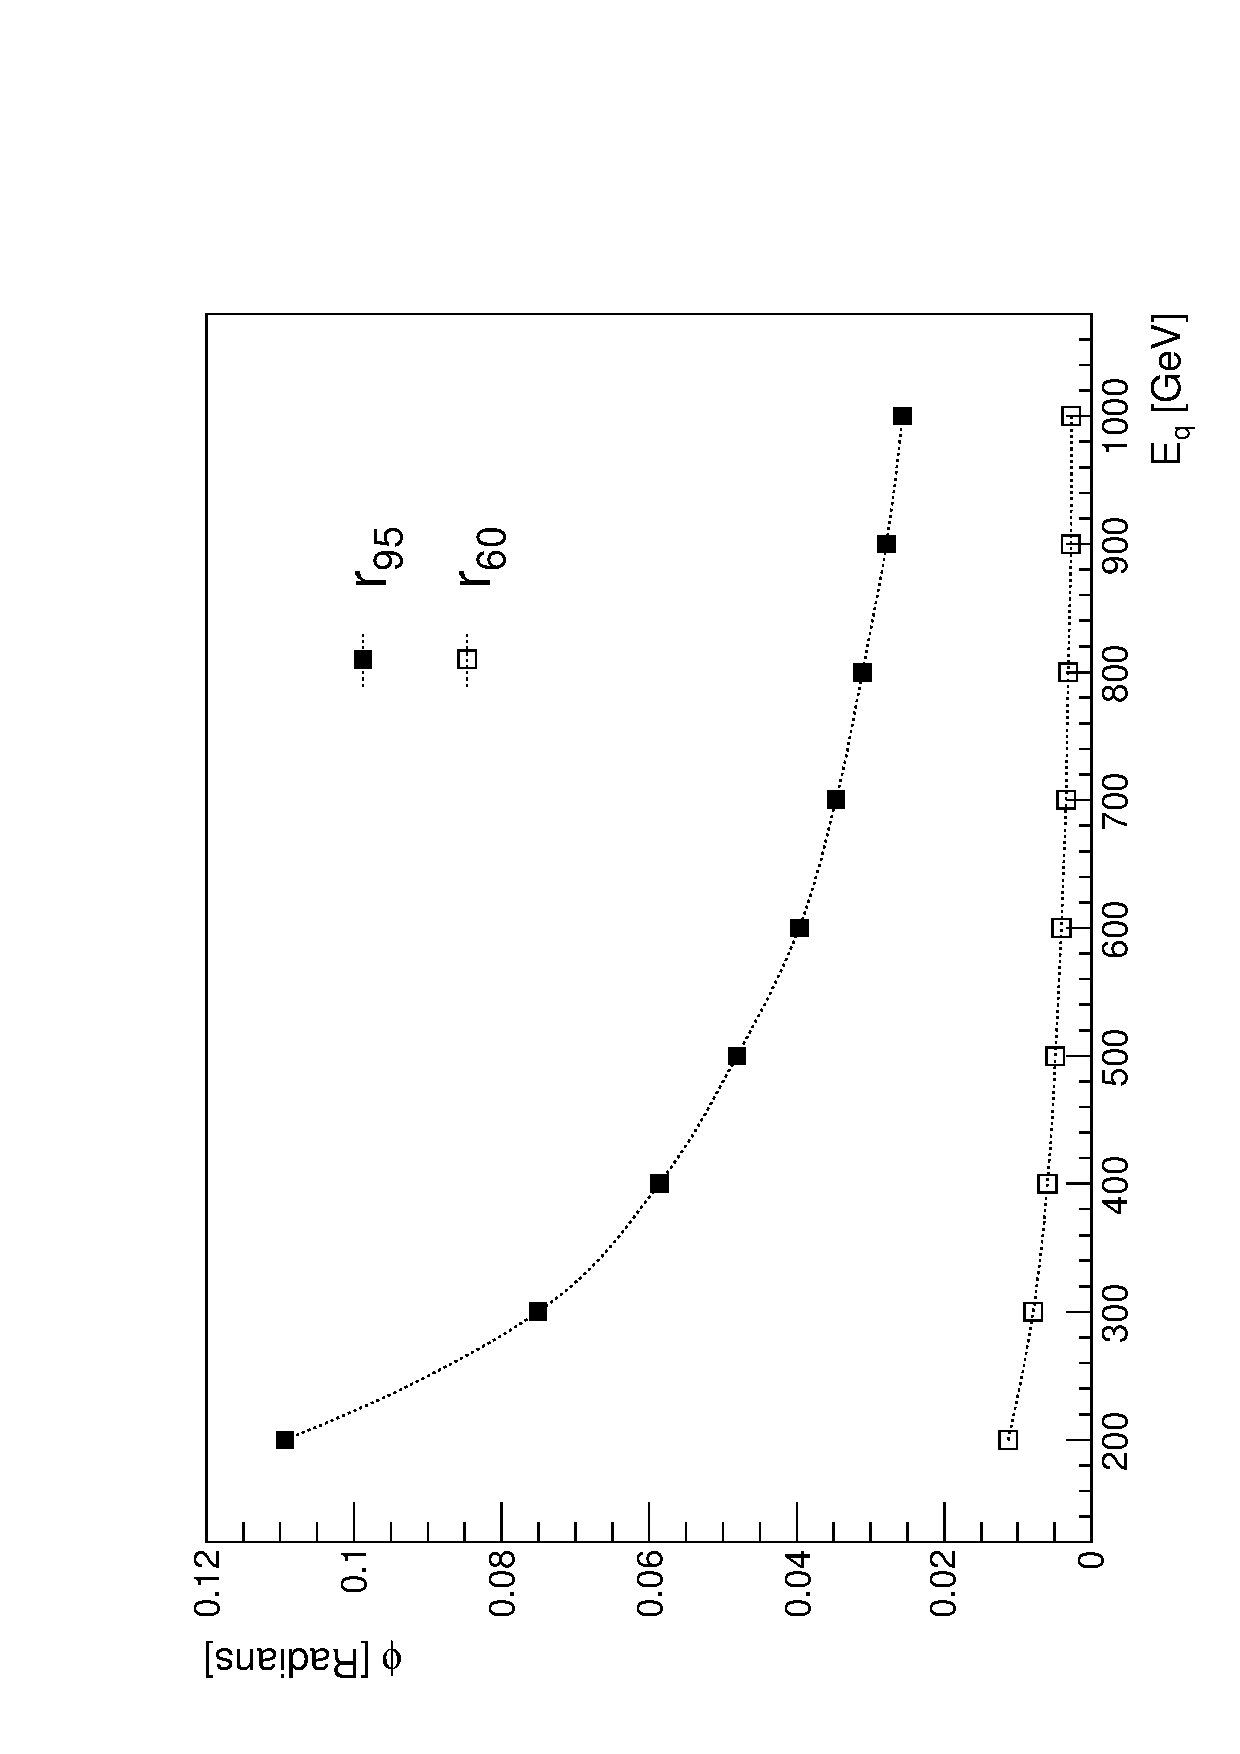
\includegraphics[width = 0.7\textwidth]{r_q.pdf}
      \caption{The 95\% and 60\% final state jet widths as a function of initial quark energy. \vspace{-0.5cm}}
      \label{r q}
    \end{center}
  \end{figure}

  \subsection{Applying the Semi-Classical jet algorithm} \label{ss sc}
 
  Now that I have developed a measure of the final state jet width,
  I can apply the SC jet algorithm to the final state particles and analyse the width of the reconstructed jets 
  in comparison to the final state jets. For the purposes of this discussion I will define an SC jet to be a jet that has
  been reconstructed by the SC jet algorithm. \\
  
  The first step is to see how accurately the SC jet algorithm is reconstructing the 4-momentum of the jet by comparing the axis and energy of the 
  SC jets to the initial quarks. In Figure \ref{scq phi} we can see that SC jets, for a jet width parameter of $R$ = 1, closely match the $\phi$ position of the initial quark, as demonstrated by
  the small mean and rms values of the distributions, showing that the SC jet algorithm performs well in reconstructing the azimuthal direction of the jet.
  Figure \ref{scq E} shows that the SC jet algorithm reconstructs energies predominantly accurately 
  with some loss of energy. This net loss of energy is demonstrated by the positive mean values, however the rms values shows that the energy loss
  is predominantly  within 20 GeV for smaller quark energies and 50 GeV for larger quark energies. The loss of energy is because the background subtracting 
  nature of the SC jet algorithm, as described in the introduction, will mean that the algorithm removes some of the actual jet constituents in some cases. This inaccuracy in 
  reconstructing the energy does not undermine the integrity of the SC jets because the effect is small for the majority of events.\\

 \begin{figure}[!htb]
    \begin{center}
      \includegraphics[width = 0.95\textwidth]{scq_phi}
      \caption{Histograms to show the difference in $\phi$ between the quark and the reconstructed \\
               SC jet axis with $R$ = 1, for different quark energies.  ($\Delta\phi = \phi_{q}-\phi_{jet}$) }
      \label{scq phi}
    \end{center}
  \end{figure}
 
  \begin{figure}[!htb]   
    \vspace{-0.5cm}
    \begin{center}
      \includegraphics[width = 0.95\textwidth]{scq_E}
      \caption{Histograms to show the difference in $E$ between the quark and the reconstructed \\
               SC jet with $R$ = 1, for different quark energies. ($\Delta E = E_{q}-E_{jet}$)}
      \label{scq E}
    \end{center}
    \vspace{-0.25cm}
  \end{figure}


  The next step is to calculate $r_{60}$ and $r_{95}$ of the SC jet, using the same technique employed for the final state jets in subsection 
  \ref{ss fs}. However, as this is profiling the width of the SC jet, one must use the SC jet's constituents, axis and energy to 
  calculate the 60\% and 95\% thresholds, instead of using the final state particles, initial quark axis and initial quark energy as before.
  The distributions of the individual $r_{95}$ and $r_{60}$ have a peak and a long tail; which is a similar shape to those 
  for the final state jets in Figure \ref{r q distr}.
  Hence, fitting with a fifth-order polynomial could be used again to interpolate the values for $r_{60}$ and $r_{95}$ at the maxima. \\

  Figure \ref{r sc} shows the $r_{95}$ and $r_{60}$ values for jets reconstructed by the SC jet algorithm with different $R$ values,
  compared to the final state jet widths calculated in subsection \ref{ss fs}. Errors are in the range 1-2\%, hence are not shown in Figure
  \ref{r sc} as the error bars are smaller than the point markers.
  The dotted lines represent an error weighted fitting of the form $r = A/(E_{jet}+B)$, where the values of the fitting parameters $A$ and $B$ 
  are given in Appendix \ref{fittings}. Figure \ref{divide sc} shows the ratio of the SC jet width to the equivalent final state jet width for 
  the $r_{60}$ and $r_{95}$ widths. \\

  \begin{figure}[!htb]
    \begin{center}
      \includegraphics[width = \textwidth]{r_sc}
      \caption{The jet widths, (a) $r_{60}$ and (b) $r_{95}$, for the final state jets compared to the jets reconstructed using the SC jet algorithm with
              varying jet width parameter, $R$. }
      \label{r sc}
    \end{center}
    \vspace{-0.5cm}
  \end{figure}
  \begin{figure}[!htb]
    \begin{center}
      \includegraphics[width = \textwidth]{divide_sc}
      \caption{The ratio for (a) $r_{60}$ and (b) $r_{95}$, of jets reconstructed using the SC jet algorithm with
              varying jet width parameter, $R$, to the equivalent final state jet width. }
      \label{divide sc}
    \end{center}
    \vspace{-0.5cm}

  \end{figure}
  
 
  Figures \ref{r sc} and \ref{divide sc} show that the SC jet algorithm reconstructs the $r_{60}$ of the jet with reasonable accuracy, particularly at high energy. 
  Figure \ref{divide sc} shows that the $r_{60}$ widths of the reconstructed jets are thinner than the final state jets by a factor of 0.7-0.9, which is due to the 
  pruning nature of the SC jet algorithm removing some of the true jet constituents. The SC jet algorithm reconstructs the $r_{95}$ width
  thinner by a factor of approximately 0.4-0.7. The notably smaller $r_{95}$ values may be due to the jet algorithm cutting off 
  significant amounts of the true jet at wide angles.
  However, one must also consider that it could be the final state jet width $r_{95}$ values 
  that are too wide, due the effect of missing quark energy discussed in the last paragraph of subsection \ref{ss fs}. 
  The cause of the seemingly anomalous bump at $700$ GeV of the $r_{95}$ is not understood and requires further analysis. However, it seems unlikely to me that it has any
  physical importance. \\
  
  Figures \ref{r sc} and \ref{divide sc} also show that the jets reconstructed using the higher values of $R$ have a more accurate jet width than those of lower $R$. 
  This is because the larger $R$ value suppresses the inter-jet distances $d_{ij}$, defined in Eq. \eqref{dij sc}, meaning that more cluster 
  mergers are allowed. 
  This observation indicates that for a free quark jet, produced by a clean channel such as $Z' \to u + \bar{u}$, a large value of $R$ ($\sim$1.5-2.0)
  should be chosen for the SC jet algorithm to optimise jet width reconstruction.
  However, there are other cases where there may be more background; such as events with more underlying event, two jets produced near each other in the final state, 
  or pile-up (which is when many events occur at roughly same time \cite{pile-up}).
  In these cases it is highly likely that a large $R$ parameter would 
  cause the reconstructed jet to include some of these non-jet events and hence the reconstructed widths would become artificially large.
  Further investigation is required for these cases. \\

  Although the fittings to the SC jet widths, in Figure \ref{r sc}, are not as strong as the fittings to the final state jet widths, as several points lie off the
  fitted line, the fittings still show that the reconstructed jets are also consistent with inverse-$p_T$ jet width narrowing. One must also note that the shape of the $r_{60}$ 
  and $r_{95}$ distributions as a function of $E$ are slightly different to that of the final state jets. This is shown in Figure \ref{divide sc}, as if the shape was the
  same, one would expect a flat line. Instead, the ratios form a linear line with a shallow positive gradient, showing that the shapes are similar but subtly different.
  This indicates that the SC jet algorithm might not accurately reconstruct jet widths with energies above and, in particular, below the range considered in this report. 

 
 \subsection{Comparison to Current Sequential Recombination Algorithms} \label{ss others}

  In this subsection I will compare the width of jets reconstructed by the SC jet algorithm to that of the anti-$k_{T}$, $k_{T}$ 
  and Cambridge-Aachen (CA) algorithms. For the purposes of this discussion, I shall collectively call anti-$k_{T}$, $k_{T}$
  and CA algorithms as the current algorithms and I shall also define an anti-$k_T$ jet, a $k_T$ jet and a CA jet to be a jet
  that has been reconstructed by its respective algorithm. \\

  Just like in subsection \ref{ss sc}, I will first compare the position and energies
  of the reconstructed jets to the initial quarks. The distributions of $\Delta\phi$ between anti-$k_{T}$, $k_{T}$ and CA jets and the initial quarks
  are very similar to that of the SC jets, which is shown in Figure \ref{scq phi}. This shows that all of the algorithms perform well in reconstructing
  the azimuthal direction of the jets. \\
  
  \begin{figure}[!htb]
    \begin{center}
      \includegraphics[width = 0.87\textwidth]{jetq_E}
      \caption{Histograms to show the difference in $E$ between the quark and the reconstructed 
               jet for different quark energies. The algorithms used were anti-$k_{T}$ (akt), $k_{T}$ (kt) 
               and Cambridge-Aachen (ca) algorithms, with $R$ =1. \vspace{-0.5cm}}
      \label{jetq E}
    \end{center}

  \end{figure}
  
  Figure \ref{jetq E} shows the difference in energy, $\Delta E$, between the initial quark and anti-$k_{T}$, $k_{T}$ and CA jets 
  at 200 and 1000 GeV. The mean and rms values of the distributions of equivalent quark energy in Figure \ref{jetq E} are similar in 
  comparison to each other, and smaller than those of the SC jet algorithm, which are shown in Figure \ref{scq E}.
  This demonstrates that the energy tagging performance of the current algorithms is similar in comparison to each other, and improved in comparison to
  the SC jet algorithm.
  One should also note that the current algorithms have considerably higher occurrence of the reconstructed jet energy being larger than 
  the quark energy. The observation of the improved energy tagging performance shows us that the current algorithms include more of the true
  jet constituents than the SC jet algorithm does, as they do not have the pruning effect of the SC jet algorithm. However, this also means that they are more susceptible to 
  including background in their reconstructions, which is shown by the observation of the increased chance of $E_{jet} > E_q$. \\

  The $r_{95}$ and $r_{60}$ values for the anti-$k_T$, $k_T$ and CA jets were then calculated using the same technique as used previously. Again the
  distributions of the individual events' $r_{95}$ and $r_{60}$ consist of a peak with a long tail; similar in shape to those shown in Figure 
  \ref{r q distr}. Hence the use of a fifth-order polynomial fitting to find the maxima is justified. Figure \ref{r all} shows the $r_{60}$ 
  and $r_{95}$ for anti-$k_{T}$, $k_{T}$ and CA jets compared to the final state jet widths. Errors are again in range 1-2\%, thus error bars 
  are not shown in Figure \ref{r all} as they are smaller than the point markers. The figure shows that the current algorithms reconstruct the 
  jet widths very similarly to each other.  As before, the dotted lines are error weighted fitted lines of the form $r = A/(E_{jet}+B)$ where 
  $A$ and $B$ are fitting parameters given in Appendix \ref{fittings}. Figure \ref{divide all} shows the ratios of the width of jets reconstructed 
  by the current algorithms to the equivalent final state jet widths for $r_{60}$ and $r_{95}$. \\

  \begin{figure}[!htb]
    \begin{center}
      \includegraphics[width = \textwidth]{r_all}
      \caption{The jet widths, $r_{60}$ and $r_{95}$ respectively, for the final state jets compared to the jets reconstructed using the anti-$k_{T}$ [(a) and (b)], 
               $k_{T}$ [(c) and (d)] and Cambridge-Aachen [(e) and (f)] jet algorithm with varying jet width parameter, $R$.}
      \label{r all}
    \end{center}
    \vspace{-0.4cm}
  \end{figure}

  For $r_{60}$ [(a), (c) and (e)] we can see that the jet width is being reconstructed wider than the final state jet width for 
  the current algorithms when a larger value of $R$ is used. This is in contrast to SC jet widths shown in Figure \ref{r sc}. This shows that, without 
  the pruning property of the SC jet algorithm, higher $R$ values will allow too much background energy to be included in the reconstruction of the jet for the current 
  algorithms, forcing the reconstructed jets to be wider.
  Hence a lower value of $R$ should be chosen, to help exclude background from the reconstruction. To optimise $r_{60}$ width reconstruction for the 
  current algorithms; a value of $R \sim 1.0$ should be chosen for jets with $E < 400$ GeV, and a width parameter of $R \sim 0.5$ should be chosen for jets with 
  $E > 400$ GeV. \\

  \begin{figure}[!htb]
    \begin{center}
      \includegraphics[width = \textwidth]{divide_all}
      \caption{The ratio of $r_{60}$ and $r_{95}$ respectively, for jets reconstructed using the anti-$k_{T}$ [(a) and (b)], 
               $k_{T}$ [(c) and (d)] and Cambridge-Aachen [(e) and (f)] with 
               varying jet width parameter, $R$, to the equivalent final state jet width.}
      \label{divide all}
    \end{center}
    \vspace{-0.4cm}
  \end{figure}
  
  Figures \ref{r all} and \ref{divide all} also show that for the $r_{95}$ jet widths, one must choose a large $R$ value ($R \sim 2.0$) to closely reconstruct the 
  width of the final state jet. However this is a very surprising result as Figure 3 of \cite{sc} shows that the current algorithms exaggerate the mass of 
  a jet for large $R$ values. Hence, we would expect that for large values of $R$ we would get artificially wide jets, as found for the $r_{60}$ widths.
  The observation that large $R$ values are required indicates that the final-state $r_{95}$ may not be a good measure of the true jet width. The widening to the 
  final state jet's $r_{95}$ could be due to the initial quark losing energy through gluon radiation, as outlined in the final paragraph of subsection \ref{ss fs}. \\

  The fittings in Figure \ref{r all}, represented by the dotted lines, are strong showing that the jets reconstructed by the current algorithms are consistent with 
  inverse-$p_T$ narrowing. 
  Graphs (a), (c) and (e) in Figure \ref{divide all} show that the shape of the distribution of $r_{60}$ values as a function of energy is different for 
  jets reconstructed by the current algorithms and final state jet widths, 
  which demonstrates that outside the energy range considered the current algorithms may not be accurate in reconstructing jet widths or a different $R$ value 
  should be used to optimise jet width reconstruction. The approximately flat lines in (b), (d) and (f) of Figure \ref{divide all} show that the distributions 
  of the $r_{95}$ values as a function of energy for the current algorithms are very similar to that of the final state jet widths. However, given the concerns 
  expressed above about the accuracy of the final state $r_{95}$ widths as a measure of the true jet width, no conclusions should be drawn from the similar $r_{95}$ distributions.\\

  One important area of further investigation required is the examination of the width properties of jets reconstructed by the current algorithms combined with
  one of the common background subtraction techniques, such as pruning. This combination of algorithm followed by pruning is commonly used in jet studies \cite{ATLAS} 
  \cite{CMS}, hence it would be important to compare the performance of the SC jet algorithm to these combinations.


  \section{Conclusions}
  
  In this report I have investigated the reconstruction of jet widths by the Semi-Classical jet algorithm compared to the other sequential recombination algorithms 
  currently in use for a range of values of jet width parameter, $R$. Monte Carlo simulations of the event $Z' \to u + \bar{u}$ were used to carry out these investigations. \\
  
  It has been shown that for the 60\% jet width, $r_{60}$, the Semi-Classical jet algorithm is effective in reconstructing jet width when $R = 1.5-2.0$. In contrast,
  the anti-$k_T$, $k_T$ and Cambridge-Aachen algorithms are effective in reconstructing jet width when $R=0.5-1.0$. It has also been shown that the distribution of widths of 
  jets reconstructed by sequential recombination algorithms as a function of energy is of the form $r = A/(E_{jet}+B)$ which is consistent with inverse-$p_T$ jet narrowing.\\

  Further studies are required to investigate the width reconstruction on events with pile-up and more background from the underlying event. 
  It is also required that the jet width reconstruction of the anti-$k_T$, $k_T$ and Cambridge-Aachen algorithms with pruning applied is 
  studied for a further comparison to the Semi-Classical jet algorithm. \\

  Another possible area of study is events where two jets are produced from a boosted object, such as in the decay of a boosted $W$ into two quarks. 
  Currently an event like this is reconstructed by applying two small $R$ sequential recombination algorithms for low energy events, to reconstruct 
  the two quark jets individually; or one large $R$ sequential recombination algorithm for the high energy cases, to reconstruct the two jets together. 
  There is an intermediate regime where neither technique is effective at reconstructing the jets. It is possible that the Semi-Classical jet algorithm, 
  as it reconstructs jet widths well at higher $R$ values, may improve performance in this intermediate regime.
  
 

\end{document}
